\chapter{Implementierung}


\section{Datenbankanwendung}

Um die Implementierung möglichst Strukturiert zu beschreiben wird hier wieder die Datenbankanwendung und der Client getrennt betrachtet.
Im folgenden Teil wird auf die Umsetzung der Architektur/Designs eingegangen, sowie auf das Zusammenspiel der Komponenten,der Layer und Funktionen.
Da Gradle als build-Tool für die Anwendung benutzt wird lassen sich alle Technologien in der Anwendung im build.gradle File wieder finden. 

\begin{figure}[h]
  \centering
  \begin{subfigure}[b]{1.0\textwidth}
    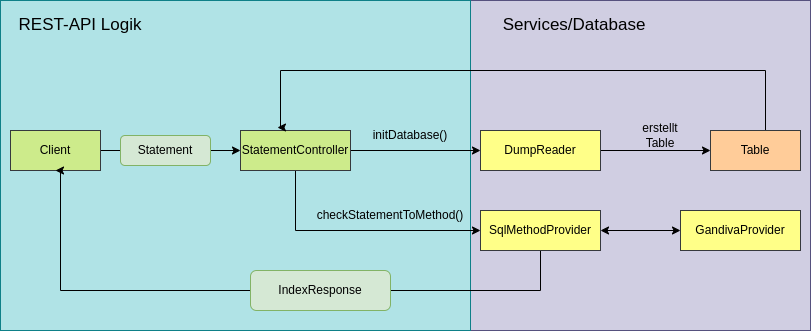
\includegraphics[width=1.0\linewidth]{img/logic}
  \end{subfigure}
  \caption{Überblick Rest-API/Services}
  \label{graf_3}
\end{figure}

\section{Komponenten}

Für den Einstiegspunkt der Datenbankanwendung ist die Initialisierung einer Datenbank nötig. Bevor jedoch auf die verschiedenen Services der Anwendung eingegangen wird, müssen vorerst die einzelnen Datenmodelle beschrieben werden. 

\subsection{Modelle}
\label{Modelle}

In der API/Datenbankanwendung existieren drei wichtige Modelle:

\begin{itemize}
 \item \textbf{Statement.java}: Dieses Modell wird als Datatransferobject behandelt. Statement enthält das SQL-Statement und wird mithilfe von Spring Boot aus dem jeweiligen Request des Clients ausgelesen und befüllt. Somit kommt über die Rest-API, die SQL-Query, in der Datenbankanwendung an und kann ausgewertet werden.
 \item \textbf{IndexResponse.java}: Wird von den verschiedenen Services, welche im folgenden Teil genauer beschrieben werden,befüllt. Das IndexResponse-Modell enthält die Speicheradressen im virtuellen Speicher und die verschiedenen Offset-Indices, falls ein Filter auf die Daten angewendet wurde. Ebenfalls enthält das Modell die verschiedenen Typen der Daten, um an die richtige Stelle im Speicher, mithilfe der Indices zu springen.
 \item \textbf{Table.java}: In diesem Modell liegen die Daten der Datenbank. Bei Initialisierung wird ein leeres VectorSchemaRoot-Objekt mithilfe eines Schemas angelegt. Dieses Objekt spiegelt das Grundgerüst der Datenbank wieder. Hier werden die Verschiedenen Spalten in Form von Vektoren gespeichert. Jeder Vektor ist einer Spalte aus dem SQL-Dump zuzuordnen.
\end{itemize}

\begin{figure}[h]
  \centering
  \begin{subfigure}[b]{1.0\textwidth}
    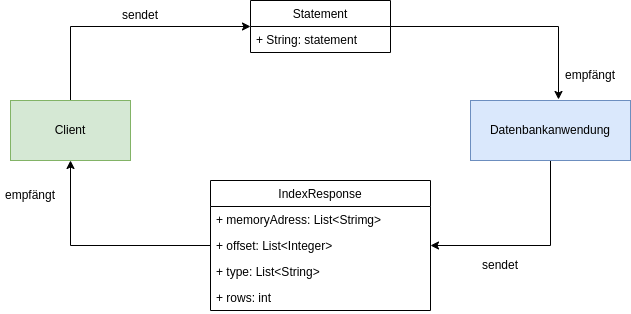
\includegraphics[width=1.0\linewidth]{img/sendrecieve}
  \end{subfigure}
  \caption{Modell-API-Kreislauf}
  \label{graf_2}
\end{figure}

Einen Überblick über das Zusammenspiel der Modelle, bzw Java-Objects, gibt uns die Abbildung \ref{graf_2}. 
Hier wird vom Client ein Statement gesendet und von der Datenbankanwendung mithilfe der Rest-API empfangen. Nach der Prozessierung des Statement erstellt die Datenbankanwendung eine IndexResponse und sendet diese dem Client zurück.
Der Client ist nun laut Theorie in der Lage über Remote Direct Memory Access auf die Stellen im Speicher zuzugreifen, welche von ihm angefragt wurden.


\section{Services}
Um eine Datenbank zu initialisieren oder ein SQL-Statement an diese schicken zu können, muss der Client, über eine Rest-API,das Backend anstoßen.
Da unter der reinen Datenbank eine Rest-API liegt, kann man über verschiedene Routen in dem \textbf{StatementController.java} diese ansteuern.


\subsection{StatementController}
Es existieren zwei wichtige Routen:

\begin{itemize}
 \item Get-Method: /initDatabase : Initialisierung eines SQL-Dumps,welcher in dem gleichen Ordner der Anwendung liegt
 \item Post-Method: /sendStatement: empfängt SQL-Statement vom Client aus und schickt eine IndexResponse zurück
\end{itemize}

Mithilfe dieser Routen kann über den StatementController in Form von einer Rest-Schnittstelle kommuniziert werden.
Wenn ein SQL-Dump über die Route initialisiert wird, erstellt der DumpReader-Service einen Table. (\ref{graf_3}). 


\subsection{DumpReader-Service}
Der DumpReader-Service ist für das lesen des SQL-Dumps zuständig. Er iteriert über jedes Statement in der Dump Datei,überprüft dieses und reagiert je noch Typ des Statements anders.
Findet man beispielsweise folgendes Statement im Kopf des SQL-Dumps,
\\

\begin{terminalblock}
  \begin{textcode}
CREATE TABLE `myTable` (
  `id` mediumint(8) unsigned NOT NULL auto_increment,
  `name` varchar(255) default NULL,
  `numberrange` mediumint default NULL,
  PRIMARY KEY (`id`)
) AUTO_INCREMENT=1;
  \end{textcode}
\end{terminalblock}

dann erkennt der DumpReader-Service das Create-Statement und legt ein neues Table-Objekt an. Dieses wird mit einem spezifischen Schema,sowie den verschiedenen Spaltenfelder und deren Typen gefüllt.
Diese Information erhält der Service aus dem SQL-Dump, wie in dem Beispiel oben.
Das Statement wird mithilfe des JSQL-Frameworks geparsed. \\

Zu diesem Zeitpunkt unterstützt der DumpReader-Service nur die Typen:

\begin{itemize}
 \item Char
 \item VarChar
 \item mediumint
\end{itemize}

Da Apache Arrow seine eigenen Datentypen besitzt muss von den SQL-Datentypen,die in dem SQL-Dump vorhanden sind, zu den jeweiligen Apache Arrow Datentypen gemapped werden. 
Dieses Mapping wird durch die Methode \textbf{prepareField(String colName, String colDataType)} erreicht.
Diese Methode kann beliebig erweitert werden um weitere Datentypen zu unterstützen.\\
Nachdem das Tableobjekt erstellt wurde, iteriert der DumpReader-Service weiter über die Statements bis er ein Insert-Statement findet. Dieses Insert-Statement ist wichtig um das Table-Objekt mit Daten zu füllen.
Ein Insert-Statement könnte beispielsweise so aussehen:\\

\begin{terminalblock}{insert.sql}
  \begin{textcode}
INSERT INTO `myTable` (`name`,`numberrange`)
VALUES
  ("Oleg Estrada",4),
  ("Bevis Davenport",0),
  ("Ronan Tucker",9);
  \end{textcode}
\end{terminalblock}

Der DumpReader-Service erkennt nun das Insert-Statement und springt in die \textbf{prepareDataForMemory(String stmt,Table table)} Methode. Hier wird wieder mithilfe von JSQL das INSERT-Statement geparsed und in Datenstücke aufgespalten.
Da bei der Initialisierung der Datenbank ein Table-Objekt mit einem VectorSchemaRoot-Objekt und einem Schema erstellt wird,können hier die Daten aus dem Insert-Statement in die dazugehörigen Vektoren geschrieben werden.
Zusätzlich wird ein Indexvektor hochgezählt,welcher den Index des Eintrags abbildet.\\\\

Wichtig zu verstehen ist, dass in der \textbf{prepareDataForMemory(String stmt,Table table)} über die einzelnen Dateneinträge aus dem Statement iteriert wird und pro Eintrag auf das VectoSchemaRoot-Objekt in dem Table-Objekt zugegriffen wird. Hier wird mit dem spezifischen Spaltennamen und Spaltentyp gearbeitet.
\\
Ein Abstraktes Beispiel für den Zugriff einer Spalte in einem VectorSchemaRoot Objekt sieht man im folgenden Codeschnipsel:\\\\

\begin{codeblock}{AbstractVectorSchemaRoot.java}{Java}
  \begin{javacode}
    ...
    FieldVector field=table.vectorSchemaRoot.getVector(colName);

    if(field instanceof IntVector){
      ((IntVector)table.vectorSchemaRoot.getVector(colName)).setSafe(table.getCounter(),Integer.parseInt(exp.get(i).toString()));
	}    
    ...
  \end{javacode}
\end{codeblock}

Zu aller erst wird über den Spaltennamen (colName) der nötige FieldVektor in eine Variable eingelesen. Dieses FieldVector-Interface kann dann auf seinen Typen mithilfe des instanceof-Operators überprüft werden. Dieser Typ wurde in dem VectorSchemaroot zuvor über die \textbf{prepareField(String colName, String colDataType)} Methode angegeben.


In dem Code-Beispiel wird also der Spaltentyp auf einen IntVector überprüft und dann der FieldVektor auf diesen IntVector-Typen gecasted, um dann mithilfe der setSafe-Methode einen Wert in den Vektor zu schreiben.
Der setSafe-Methode wird ebenfalls ein Index mitgegeben um  die richtige Spalte in dem Table bzw. Vektor zu befüllen. Dieser Index wird im Table-Objekt,wie in dem Modell beschrieben, überprüft und inkrementiert.
\\
Das FieldVector-Interface wird von einigen Datenklassen im package org.apache.arrow.vector implementiert, sodass eine große Auswahl an Datentyp-Möglichkeiten existieren. Falls nicht der richtige Datentyp gefunden wird, kann eine eigene Klasse implementiert werden, welche den eigenen Anforderungen entsprechen und das Interface FieldVector implementiert.
Die Anwendung unterstützt momentan die Datentypen IntVector und VarCharVector.
\\
Der DumpReader kümmert sich letztendlich um die Initialisierung eines SQL-Dumps und das Mapping zwischen den SQL-Datentypen und den Apache-Arrow Datentypen. Er ist der dafür verantwortlich ein Table-Objekt zu erstellen und diesem Daten  in Form von Apache Arrow Vektoren zuzuweisen.
Über das Table-Objekt werden schließlich die Daten auf Anfrage ausgewertet.





\subsection{SqlMethodProvider-Service}
\label{SqlMethodProvider-Service}
Anfragen über die Datenbank laufen vom StatementController aus in den SqlMethodProvider-Service. Dieser ist dafür zuständig das SQL-Statement und somit die Datenanfrage auszuwerten.

Alle Anfragen in Form von Statements werden von einer Verteiler-Methode aus an weitere Methoden verteilt und vom Statement abhängig ausgewertet.
Die Verteiler-Methode \textbf{checkStatementToMethod(String statement, Table table)} bekommt das Statement als String, sowie das Table-Objekt aus dem DumpReader-Service übergeben. In der Arbeit wird nur mit einem Table gearbeitet, somit findet hier keine Logik für die Auswahl eines Tables statt. Jedoch lässt sich dieses Feature einfach erweitern. Weiteres dazu in Abschnitt Erweiterungen.\\

In der Verteiler-Methode wird das Statement mit JSQL in verschiedensten Ausführungen geparsed. Diese Ausführungen sind von dem gewollten Datenanfrage-Umfang abhängig.Der folgende Unterabschnitt geht weiter auf die einzelnen Handmade-Methoden ein, die mit den Kern der Anwendung ausmachen.


\subsubsection{Handmade-Methoden}


Es wird zwischen zwei Arten von Methoden unterschieden an die verteilt wird,da einige Anfrage-Fälle einfacher umgesetzt werden können als andere.
Die Handmade-Methoden benutzen keine weiteren Services,um die Datenbankauswertung anzustoßen. Im Gegensatz dazu wird bei komplexeren Anfragen der GandivaProvider-Service benutzt,um die Daten in der Datenbank zu filtern.
Alle Methoden liefern jedoch ein einheitlich ein IndexResponse-Objekt als Antwort zurück.\\\\

\begin{codeblock}{SqlMethodProvider.java}{Java}
  \begin{javacode}
    ...
net.sf.jsqlparser.statement.Statement jsqlStatement = CCJSqlParserUtil.parse(statement.getStatement()); 

if(jsqlStatement instanceof Select) {

            Select select = (Select) jsqlStatement;
            PlainSelect plainSelect = (PlainSelect)select.getSelectBody();
            List<SelectItem> selectItemList = plainSelect.getSelectItems();

            SelectItem firstItem = selectItemList.get(0);
			...
            if(firstItem instanceof AllColumns){
                return selectEverything(table);
            }
}
    ...
  \end{javacode}
\end{codeblock}


Dieser Codeschipsel stammt aus der zuvor erwähnten Verteiler-Methode. In Zeile 2  wird ein übergebener Statement-String in ein JSQL-Statement-Objekt transferiert. Dieses Objekt lässt sich wiederum über den Klassen-Typen auswerten (Zeile 4).Nach der Auswertung wird das jsqlStatement-Objekt auf einen bestimmten Klassen-Typen überprüft. Falls das Statement ein Select-Statement darstellt muss inspiziert werden auf welche Spalten in der Datenbank zugegriffen werden soll.\\ 
Dieser Bereich der Verteiler-Methode würde bei folgendem übergebenen Statement eingreifen:

\begin{center}
\code{SELECT * FROM table;}
\end{center}

Hier wird wie oben erwähnt an die dazugehörige Handmade-Methode selectEverything(table) verteilt. Diese Art von Implementierung ermöglicht es Modular weitere Fälle abzudecken.
In der Methode selectEverything(Table table) werden alle nötigen Felder für die IndexResponse befüllt. Hierzu wird über das Table-Objekt die FieldVector-Liste ermittelt, welche alle Daten enthält. Dann werden die verschiedenen Data-Buffer-Adressen der einzelnen Vektoren ermittelt und in eine Liste geschrieben. Ebenfalls wird eine Liste mit den dazugehörigen Vektor-Typen erstellt.Für ein besseres Verständnis hilft es sich hier nocheinmal das IndexResponse-Objekt in Abschnitt \ref{Modelle} anzuschauen.\\
Da in dieser Art von Anfrage alle Einträge benötigt werden, existieren hier keine Offsets, da von der virtuellen Memory-Adresse aus mithilfe des Datentyps inkrementiert werden kann.Dafür wird die Anzahl der Einträge, welche die Anfrage widerspiegelt mit übergeben.In diesem Fall bleibt die Offset-Liste also leer.
Somit wird ein valide IndexResponse generiert und es kann vom Client auf die angefragten Daten per RDMA zugegriffen werden.Die an den Client übermittelte IndexResponse wird über den Controller in Form von JSON zurückgeliefert. Dies kann man sehr gut in der Grafik \ref{graf_4} erkennen.

\begin{figure}[h]
  \centering
  \begin{subfigure}[b]{0.5\textwidth}
    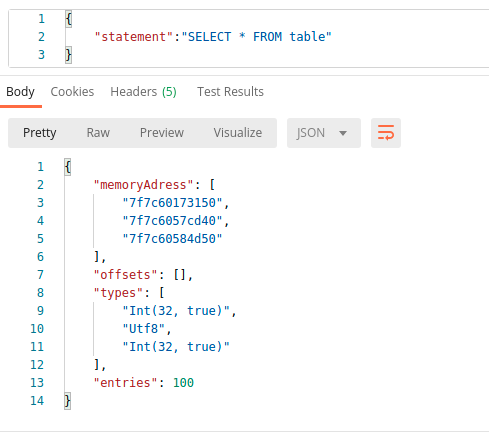
\includegraphics[width=1.0\linewidth]{img/json}
  \end{subfigure}
  \caption{JSON Anfrage (Statement) und Antwort (IndexResponse)}
  \label{graf_4}
\end{figure}

In der Anwendung existieren momentan zwei Handmade-Methode. Auf eine davon wurde nun bereits eingegangen.Die zweite Methode ist die Methode selectEverythingFromCols(List<String> colNames,Table table). Für diese Methode wird kein Gandiva Filter benötigt, daher ist sie von Hand geschrieben und wird in dieser Arbeit ebenfalls Handmade-Methode genannt.

Diese Methode wird bei einem Statement mit Zugriff auf spezifische ganze Spalten in der Datenbank ausgeführt. Hier wird sich beispielsweise das Statement   

\begin{center}
\code{SELECT spalte1,spalte2 FROM table;}
\end{center}

angeschaut und die spalte1 und spalte2 im VectorSchemaRoot-Objekt des Tables gesucht, um dann wiederum die nötigen Daten für die IndexResponse zu bauen.
In der IndexResponse werden dann nur die virtuellen Memory-Adressen zurückgeliefert, welche zu den ausgewählten Spalten gehören.
In diesem Fall würde es in der Grafik \ref{graf_4} unter dem Feld memoryAdress nur zwei Einträge geben.

\subsection{GandivaProvider-Service}

Wie in \ref{SqlMethodProvider-Service} bereits erklärt, gibt es im Sql-MethodProvider-Service nicht nur Handmade-Methoden sondern auch Methoden die mit dem GandivaProvider-Service zusammenhängen.
\\
Sobald ein Statement übergeben wird, welches nur spezifisch ausgewählte Daten der Datenbank beansprucht,wird das Framework Gandiva in Betracht gezogen.
Im weiteren Verlauf dieses Abschnitt werden auf komplexere Beispiele in Bezug auf das Gandiva-Framework eingegangen. Die Grundlegende Funktion von Gandiva kann in Abschnitt \ref{Gandiva} nachgelesen werden.

Sobald die Verteiler-Methode erkennt, dass Gandiva für das Statement benötigt wird, springt dieser in die zuständige GandivaProvider-Methode und übergibt abhängig von der Operation verschiedene Parameter. Zur Veranschaulichung wird hier auf ein Code-Beispiel eingegangen.

\begin{codeblock}{SqlMethodProvider.java}{Java}
  \begin{javacode}
    private IndexResponse selectWhereEqualsTo(String columnName, int value, Table table) throws GandivaException {

        Filter filter = gandivaProvider.equalsTo_NumberFilter(table,columnName,value);

        ArrowRecordBatch batch = gandivaProvider.createBatch(table,columnName);

        SelectionVectorInt32 selectionVectorInt32 = gandivaProvider.createSelectionVector(table);

        filter.evaluate(batch,selectionVectorInt32);

        int[] indices = MemoryUtil.selectionVectorToArray(selectionVectorInt32);

...

  \end{javacode}
\end{codeblock}

Diese Methode selectWhereEqualsTo wird beispielsweise durch das Statement

\begin{center}
\code{SELECT spalte FROM table WHERE spalte = 5}
\end{center}

ausgeführt. Hier wird die Spalte spalte in der Datenbank nach dem Wert 5 gefiltert. Dieser Filterprozess wird eingeleitet durch den GandivaProvider.
Für jeder Art von Filter muss in dem GandivaProvider eine eigene Methode hinzugefügt werden. In dem GandivaProvider findet sich zum Beispiel die \textbf{equalsTo\_NumberFilter}-Methode, welche den passenden Filter generiert.
Mithilfe dieses Filters wird dann in Zeile 9 der Datensatz evaluiert. Um diesen Datensatz jedoch evaluieren zu können benötigt die Methode \textbf{evaluate} noch einen ArrowRecordBatch und einen SelectionVectorInt32.
Der ArrowRecordBatch und der SelectionVectorInt32 werden beide durch den GandivaProvider erstellt mithilfe der Methode \textbf{createBatch} und \textbf{createSelectionVector}.

\subsubsection{GandivaProvider: equalsTo\_NumberFilter}

\subsubsection{ArrowRecordBatch}

Der ArrowRecordBatch bekommt die Anzahl der Vektoren des Tables mit übergeben.
Es werden zwei ArrowBuffer erstellt. In dem Spalten-Buffer werden die nötigen Daten des Vektors bzw der Spalte abgelegt und in dem Validity-Buffer wird festgelegt welche Einträge der Spalten valide Einträge sind. Das heißt hier könnte man wenn man möchte Spalteneinträge aus der Datenbankanfrage ausschließen.
Diese beiden ArrowBuffer werden in einer Liste verpackt und in dem Konstruktor des ArrowRecordBatch übergeben. Zusätzlich wird noch eine Liste übergeben mit ArrowFieldNodes, welche die ganze Spalten ausschließen kann. In dem oben genannten Beispiel wird diese Funktion nicht benötigt.

\subsubsection*{SelectionVector32}

Der SelectionVector stellt eine Repräsentation eines ArrowBuffers dar, welcher groß genug ist um die ausgewerteten Daten der Evaluation festzuhalten.



- Wie erweitere ich die Anwendung
- Wie schnell liefert mir eine Anfrage den Zugriff
- Was kann ich zu den Daten sagen
- Wie funktioniert Gandiva
- CheckStatementToMethod auf Table-Spezifisch erweitern


